\begin{figure}[tp]
\centering
\begin{minipage}{\textwidth}\noindent\textbf{A}\par\vspace{-0.3em}
\begin{tikzpicture}
\begin{axis}[
  width=0.79\textwidth, height=5.4cm,
  axis lines*=left,
  xmode=log,
  xmin=0.0001, xmax=0.85, ymin=0.48, ymax=0.68,
  xtick={0.0001, 0.01, 0.1, 0.85},
  xticklabels={0.0001, 0.01, 0.1, 0.85},
  ytick={0.5, 0.55, 0.6, 0.65},
  yticklabels={even, 0.55, 0.60, 0.65},
  xlabel={compounding rate $\epsilon$},
  ylabel={center of mass of spending},
  ylabel style={font=\small}, xlabel style={font=\small},
  tick label style={font=\small},
  axis line style={line width=0.4pt},
  tick style={line width=0.4pt, black},
  clip=false,
]
\addplot[gray, dashed, line width=0.4pt, domain=0.0001:0.85] {0.5};
\addplot[black, line width=0.7pt] table[x=eps, y=rich] {fig8-boundary.dat};
\addplot[black, line width=0.7pt] table[x=eps, y=mid]  {fig8-boundary.dat};
\addplot[black, line width=0.7pt] table[x=eps, y=poor] {fig8-boundary.dat};
\node[font=\small, anchor=west] at (axis cs:0.92,0.652) {many resources};
\node[font=\small, anchor=west] at (axis cs:0.92,0.566) {intermediate};
\node[font=\small, anchor=west] at (axis cs:0.92,0.521) {few resources};
\end{axis}
\end{tikzpicture}
\end{minipage}\par\vspace{0.9em}
\begin{minipage}{\textwidth}\noindent\textbf{B}\par\vspace{-0.3em}
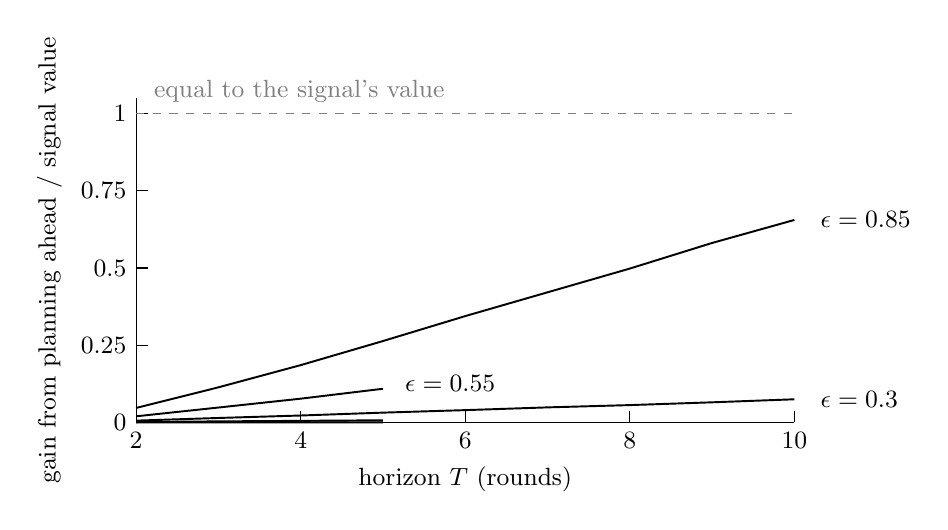
\begin{tikzpicture}
\begin{axis}[
  width=0.82\textwidth, height=5.7cm,
  axis lines*=left,
  xmin=2, xmax=10, ymin=0, ymax=1.05,
  xtick={2, 4, 6, 8, 10},
  ytick={0, 0.25, 0.5, 0.75, 1},
  yticklabels={0, 0.25, 0.5, 0.75, 1},
  xlabel={horizon $T$ (rounds)},
  ylabel={gain from planning ahead / signal value},
  ylabel style={font=\small}, xlabel style={font=\small},
  tick label style={font=\small},
  axis line style={line width=0.4pt},
  tick style={line width=0.4pt, black},
  clip=false,
]
\addplot[gray, dashed, line width=0.4pt, domain=2:10] {1};
\node[font=\small, gray, anchor=south west] at (axis cs:2.1,1.005) {equal to the signal's value};
\addplot[black, line width=0.7pt] coordinates {(2,0.0468) (3,0.1136) (4,0.1855) (5,0.2635) (6,0.3443) (7,0.4213) (8,0.4982) (9,0.5811) (10,0.6556)};
\addplot[black, line width=0.7pt] coordinates {(2,0.0198) (3,0.0482) (4,0.0769) (5,0.1090)};
\addplot[black, line width=0.7pt] coordinates {(2,0.0058) (3,0.0144) (4,0.0224) (5,0.0317) (6,0.0398) (7,0.0487) (8,0.0561) (9,0.0651) (10,0.0749)};
\addplot[black, line width=0.7pt] coordinates {(2,0.0012) (3,0.0034) (4,0.0051) (5,0.0069)};
\addplot[black, line width=0.7pt] coordinates {(2,0.0000) (3,0.0002) (4,0.0001) (5,0.0000)};
\node[font=\small, anchor=west] at (axis cs:10.2,0.656) {$\epsilon = 0.85$};
\node[font=\small, anchor=west] at (axis cs:5.15,0.126) {$\epsilon = 0.55$};
\node[font=\small, anchor=west] at (axis cs:10.2,0.075) {$\epsilon = 0.3$};
\end{axis}
\end{tikzpicture}
\end{minipage}\par\vspace{0.9em}
\caption{Strategic timing of funding. (\textit{A}) The compounding rate, not the scarcity of baseline resources, sets how far spending shifts toward later rounds: the center of mass of spending (0.5 is even; higher is later) as the compounding rate $\epsilon$ increases, for three baseline resource scales. (\textit{B}) Choosing whom outweighs choosing when: the gain from planning ahead, as a share of the review signal's value, by horizon and compounding rate; in every setting the gain is below the signal's value. Settings: \ref{app:simulation}.}
\label{fig:p3}
\end{figure}
